% !TEX root = ../../../main/aws_chabauty.tex
\newpage
\subsection{Lecture 2}

% Correction to previous lecture???

Excuse the laziness, typesetting will come later for this lecture\dots

	\begin{figure}[!ht]
	\centering
	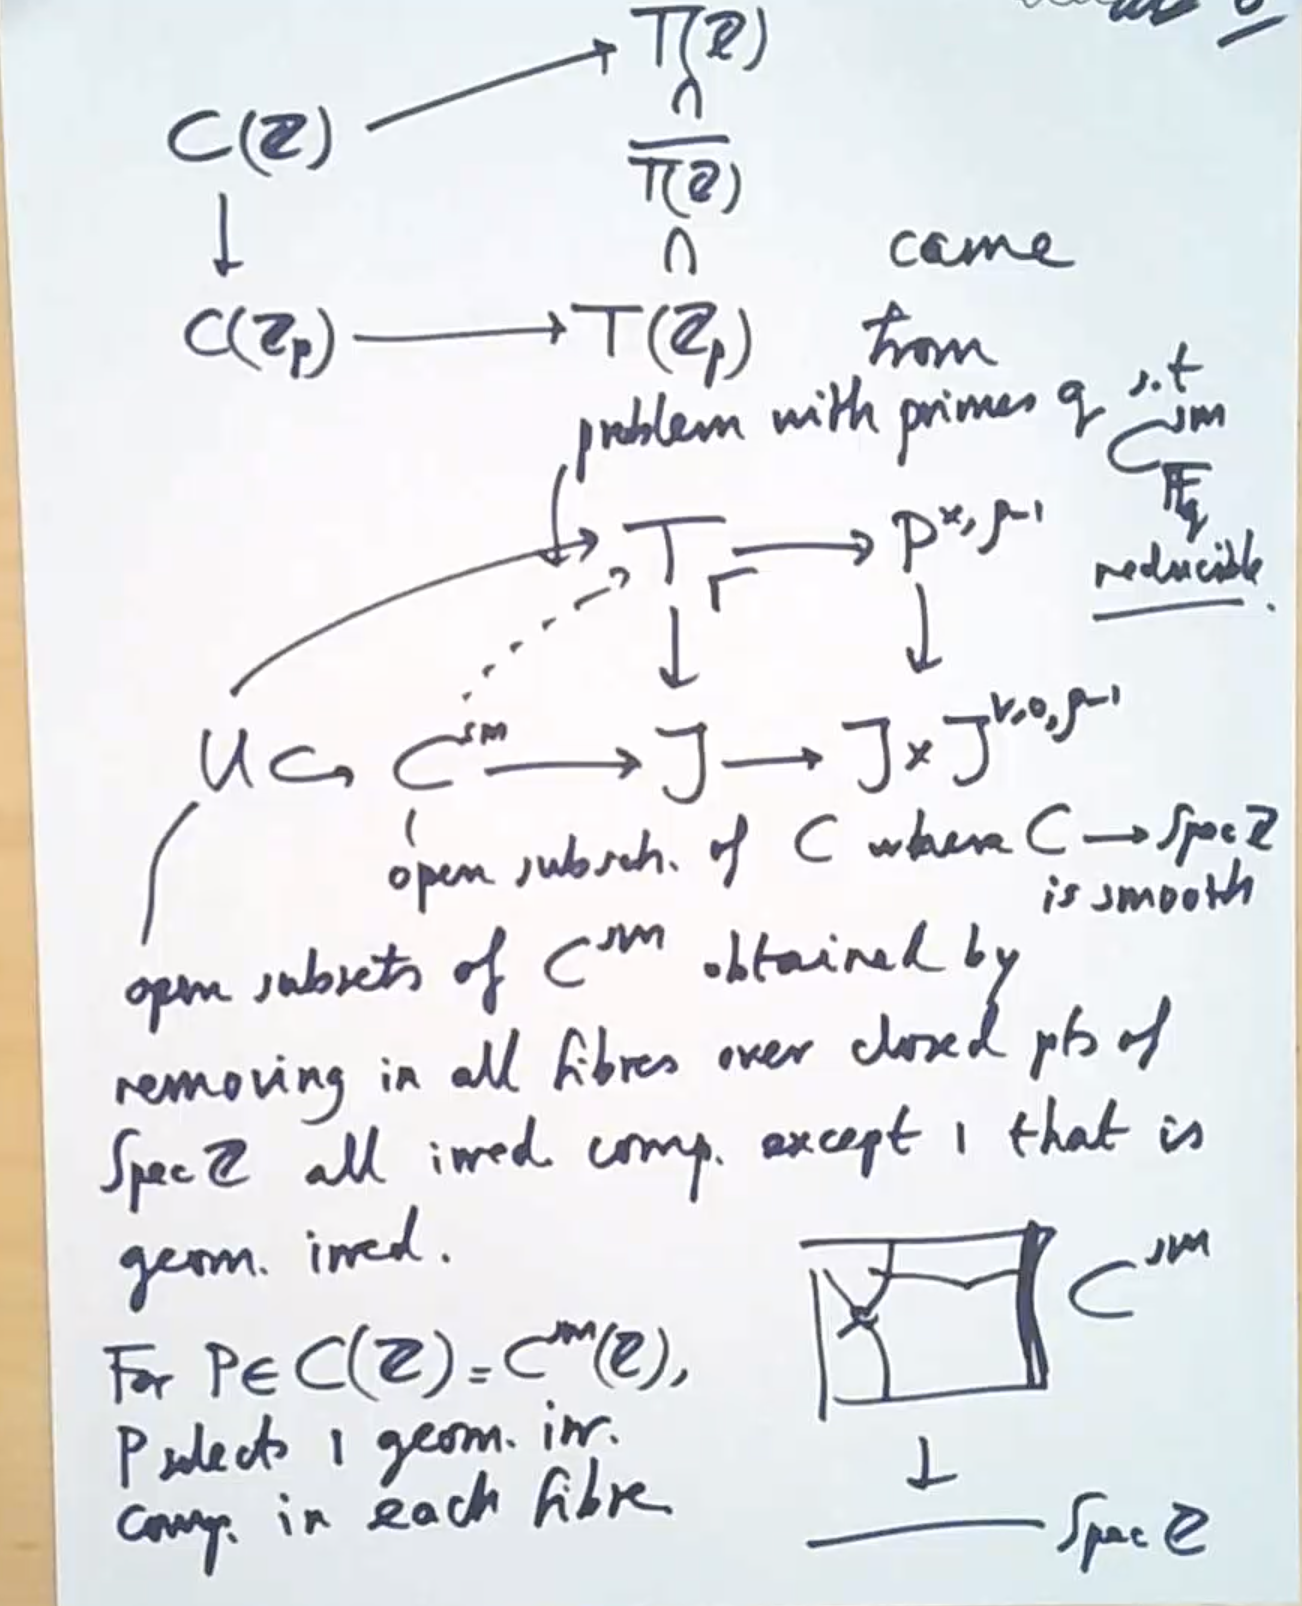
\includegraphics[width=0.5\textwidth]{../images/im12.png}
	\end{figure}


Say $n$ is the product of primes $q$ of bad reduction of $C/\Z$. Then $C \to \spec \Z$ is smooth over $\Z[1/n]$. These are finitely many of smooth $U$'s and $C_\Q= C^\text{sm}(\Z)= \sqcup_{\text{all }U\text{'s}} U(\Z)$.


\begin{ex}
$y^2+y= x^6 + \cdots$ (see section 8 of the notes). $n=3.43$, $C_{\F_{49}}^\text{sm}$ ind $C_{\F_j}^\text{sm}$. There are exactly 2 $U$'s.
	\begin{figure}[!ht]
	\centering
	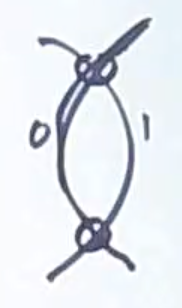
\includegraphics[width=0.1\textwidth]{../images/im13.png}
	\end{figure}
\end{ex}


	\begin{figure}[!ht]
	\centering
	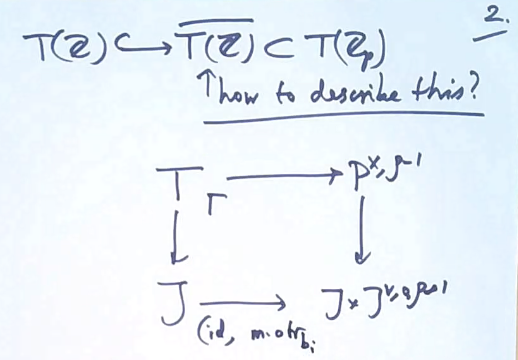
\includegraphics[width=0.5\textwidth]{../images/im14.png}
	\end{figure}


$J^{\vee,0} \hra J^\vee \twoheadrightarrow \Phi^\vee$, the group scheme of components of $J^\vee$. $\Phi^\vee$ trivial over $\Z[1/n]$. Finite \et fibers over $\Z/n\Z$. $m:=$ least common multiple of exponents of $\Phi^\vee(\tilde{\F}_q), q \mid n$. 


	\begin{figure}[!ht]
	\centering
	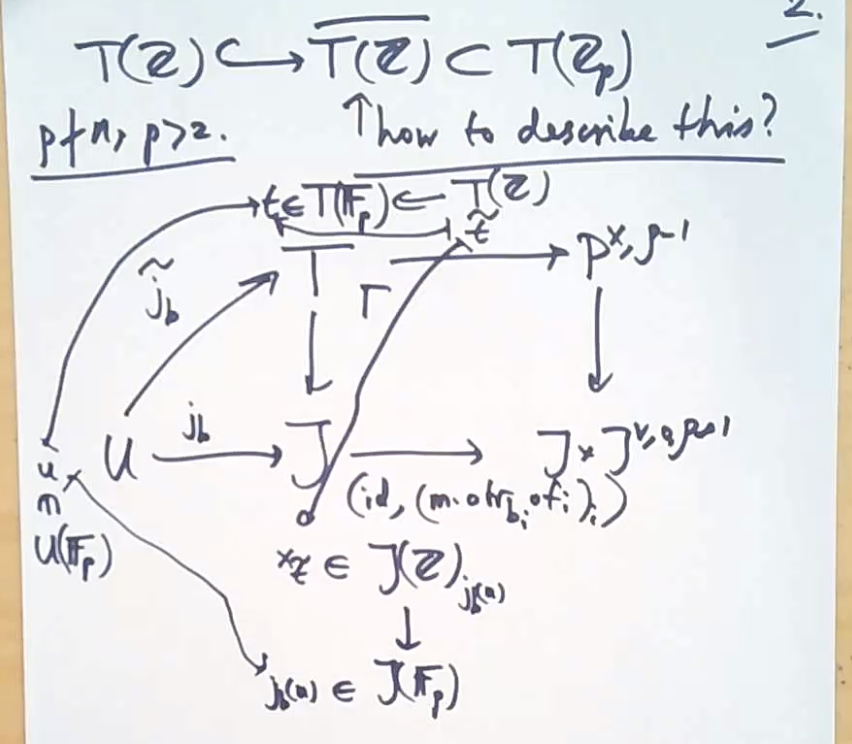
\includegraphics[width=0.5\textwidth]{../images/im15.png}
	\end{figure}


We want to create a map $J(\Z) \to T(\Z)$ but this is difficult because no such map comes from geometry. $J(\Z)_0 \cong \Z^r$, $x_1, \ldots, x_r$. We get a map $k_\Z: \Z^r \to T(\Z)_t$, not really surjective.


\begin{thm}[4.10]
	\[
	\Z^r \ma{k_\Z} T(\Z_p)_t \ma{\sim} \Z_p^{g+\rho-1}
	\]
where the bijection is given by evaluation at $1/p$ in the parametrization of $\O_{T,t}$. Note that $\Z^r \subset \Z_p^r$ is dense. There exists a unique $k=(k_1,\ldots,k_{g+\rho-1})$, $k_i \in \Z_p \langle z_1,\ldots,z_r \rangle= \Z_p[z_1,\ldots,z_r]^{\wedge p}$ and $\ov{T(\Z)}_t$ is the image of $k$. 
\end{thm}

\pf All of section 5, three and a half pages and lots of representations, $n \mapsto nP = \exp(n \log P)$. \qed \\


	\begin{figure}[!ht]
	\centering
	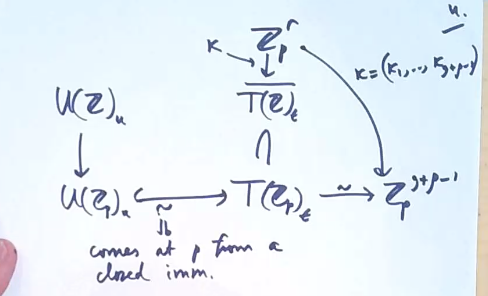
\includegraphics[width=0.5\textwidth]{../images/im16.png}
	\end{figure}


\begin{enumerate}[1.]
\item We want to pull back expressions fro the complete intersection $U \hra T$ and at $u$ get $g+\rho-2$ equations to $\Z_p^r$. 
\item We want to do this in terms of formal geometry, e.g. rings like $\Z_p \langle z_1,\ldots,z_r \rangle$, and then reduce $\mod p$, so we get polynomials in $\F_p[z_1,\ldots,z_r]$.
\end{enumerate}






















